\documentclass[8pt,aspectratio=169]{beamer}
\usetheme{Madrid}
\usepackage{graphicx}
\usepackage{booktabs}
\usepackage{adjustbox}
\usepackage{multicol}
\usepackage{amsmath}
\usepackage{amssymb}
\usepackage{tikz}
\usetikzlibrary{arrows.meta,positioning,shapes.callouts,shapes.geometric,decorations.pathreplacing}
\usepackage{hyperref}
\usepackage{algorithm}
\usepackage{algorithmic}

% Color definitions
\definecolor{mlblue}{RGB}{0,102,204}
\definecolor{mlpurple}{RGB}{51,51,178}
\definecolor{mllavender}{RGB}{173,173,224}
\definecolor{mllavender2}{RGB}{193,193,232}
\definecolor{mllavender3}{RGB}{204,204,235}
\definecolor{mllavender4}{RGB}{214,214,239}
\definecolor{mlorange}{RGB}{255, 127, 14}
\definecolor{mlgreen}{RGB}{44, 160, 44}
\definecolor{mlred}{RGB}{214, 39, 40}
\definecolor{mlgray}{RGB}{127, 127, 127}

% Additional colors for template compatibility
\definecolor{lightgray}{RGB}{240, 240, 240}
\definecolor{midgray}{RGB}{180, 180, 180}

% Backward compatibility: uppercase color names
\colorlet{MLPurple}{mlpurple}
\colorlet{MLBlue}{mlblue}
\colorlet{MLOrange}{mlorange}
\colorlet{MLGreen}{mlgreen}
\colorlet{MLRed}{mlred}
\colorlet{MLLavender}{mllavender}
\colorlet{MLGray}{mlgray}

% Apply custom colors to Madrid theme
\setbeamercolor{palette primary}{bg=mllavender3,fg=mlpurple}
\setbeamercolor{palette secondary}{bg=mllavender2,fg=mlpurple}
\setbeamercolor{palette tertiary}{bg=mllavender,fg=white}
\setbeamercolor{palette quaternary}{bg=mlpurple,fg=white}

\setbeamercolor{structure}{fg=mlpurple}
\setbeamercolor{section in toc}{fg=mlpurple}
\setbeamercolor{subsection in toc}{fg=mlblue}
\setbeamercolor{title}{fg=mlpurple}
\setbeamercolor{frametitle}{fg=mlpurple,bg=mllavender3}
\setbeamercolor{block title}{bg=mllavender2,fg=mlpurple}
\setbeamercolor{block body}{bg=mllavender4,fg=black}

% Remove navigation symbols
\setbeamertemplate{navigation symbols}{}

% Clean itemize/enumerate
\setbeamertemplate{itemize items}[circle]
\setbeamertemplate{enumerate items}[default]

% Reduce margins for more content space
\setbeamersize{text margin left=5mm,text margin right=5mm}

% Custom course footer
\setbeamertemplate{footline}{
  \leavevmode%
  \hbox{%
    \begin{beamercolorbox}[wd=.333333\paperwidth,ht=2.25ex,dp=1ex,center]{author in head/foot}%
      \usebeamerfont{author in head/foot}Methods and Algorithms
    \end{beamercolorbox}%
    \begin{beamercolorbox}[wd=.333333\paperwidth,ht=2.25ex,dp=1ex,center]{title in head/foot}%
      \usebeamerfont{title in head/foot}MSc Data Science
    \end{beamercolorbox}%
    \begin{beamercolorbox}[wd=.333333\paperwidth,ht=2.25ex,dp=1ex,right]{date in head/foot}%
      \usebeamerfont{date in head/foot}\insertframenumber{} / \inserttotalframenumber\hspace*{2ex}
    \end{beamercolorbox}}%
  \vskip0pt%
}

% Command for bottom annotation (Madrid-style)
\newcommand{\bottomnote}[1]{%
\vfill
\vspace{-2mm}
\textcolor{mllavender2}{\rule{\textwidth}{0.4pt}}
\vspace{1mm}
\footnotesize
\textbf{#1}
}

% Custom commands for course compatibility
\newcommand{\highlight}[1]{\textcolor{mlorange}{\textbf{#1}}}
\newcommand{\mathbold}[1]{\boldsymbol{#1}}

\title[L05: PCA \& t-SNE Ultra-Deep]{PCA \& t-SNE: Ultra-Deep Visuals}
\subtitle{20 Advanced Charts for the Curious Data Scientist}
\author{Prof.\ Dr.\ J\"org Osterrieder}
\institute{Methods and Algorithms --- MSc Data Science}
\date{Spring 2026}

\begin{document}

% ============================================================
% FRONT MATTER
% ============================================================

% SLIDE 1: Title Page
\begin{frame}
\titlepage
\end{frame}

% SLIDE 2: Opening XKCD
\begin{frame}[t]{The Art of Fitting}
\vspace{0.5em}
\begin{center}
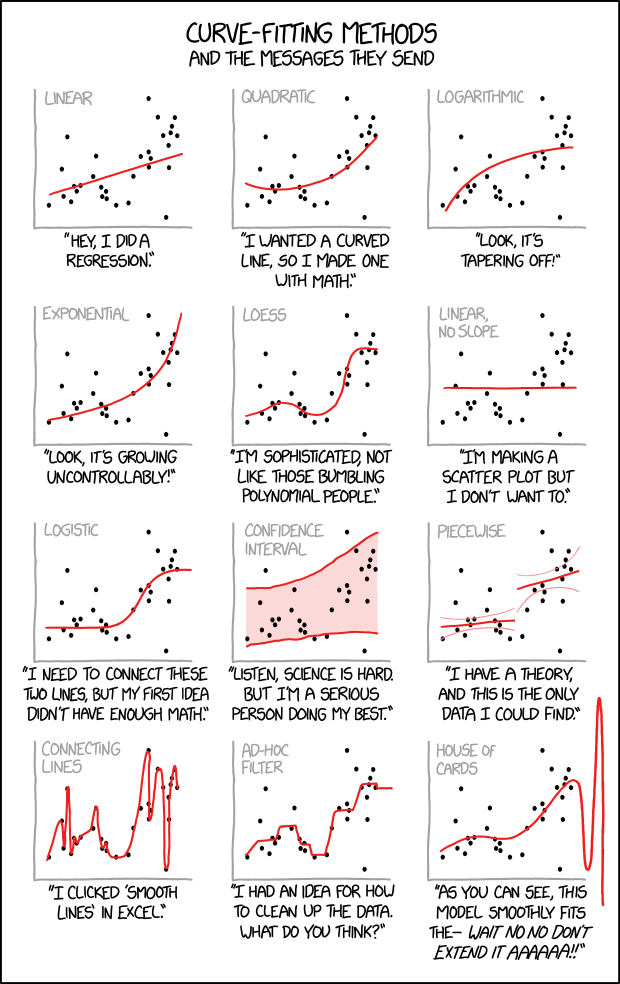
\includegraphics[height=0.55\textheight]{images/2048_curve_fitting.png}
\end{center}
\bottomnote{XKCD \#2048 by Randall Munroe (CC BY-NC 2.5)}
\end{frame}

% SLIDE 3: Learning Objectives
\begin{frame}[t]{Learning Objectives}
\vspace{1em}
After this lecture, you will be able to:
\begin{itemize}
  \item \textbf{Diagnose} PCA anomalies using Hotelling $T^2$ and SPE statistics
  \item \textbf{Evaluate} t-SNE embedding quality via trustworthiness and KL divergence diagnostics
  \item \textbf{Compare} dimensionality reduction methods for suitability on different data structures
  \item \textbf{Apply} PCA/t-SNE to realistic finance scenarios (yield curves, portfolios, credit risk)
\end{itemize}
\bottomnote{We cover 20 advanced visualizations spanning PCA diagnostics, t-SNE mechanics, practical pipelines, and finance applications}
\end{frame}

% SLIDE 4: Table of Contents
\begin{frame}{Outline}
  \tableofcontents
\bottomnote{Four parts: PCA Deep Mechanics, t-SNE Deep Mechanics, Practical Diagnostics, Finance Applications}
\end{frame}

% ============================================================
% SECTION 1: PCA DEEP MECHANICS (6 charts)
% ============================================================
\section{PCA Deep Mechanics}

% SLIDE 5
\begin{frame}[t]{Can PCA Detect Outliers? The Hotelling $T^2$ Statistic}
\begin{center}

\includegraphics[width=0.65\textwidth]{top20_21_hotelling_t2_outlier/chart.pdf}
\end{center}
\bottomnote{Hotelling $T^2$ measures Mahalanobis distance in PC space---points beyond the 99\% ellipse are statistically anomalous}
\end{frame}

% SLIDE 6
\begin{frame}[t]{What PCA Misses: The Q-Residual (SPE) Statistic}
\begin{center}

\includegraphics[width=0.65\textwidth]{top20_22_spe_q_residual/chart.pdf}
\end{center}
\bottomnote{SPE detects anomalies invisible in PC space---deviations in directions PCA discards as noise}
\end{frame}

% SLIDE 7
\begin{frame}[t]{Sparse PCA: Can We Get Interpretable Components?}
\begin{center}

\includegraphics[width=0.65\textwidth]{top20_23_sparse_pca_loadings/chart.pdf}
\end{center}
\bottomnote{Sparse PCA trades variance explained for interpretability---each component loads on only a handful of features}
\end{frame}

% SLIDE 8
\begin{frame}[t]{How Sensitive Is PCA to Outliers?}
\begin{center}

\includegraphics[width=0.65\textwidth]{top20_24_robust_pca_outlier_influence/chart.pdf}
\end{center}
\bottomnote{Just 5\% contamination can rotate PC1 by 20+ degrees---always inspect for outliers before running PCA}
\end{frame}

% SLIDE 9
\begin{frame}[t]{How Does the Number of Components Affect Cluster Separability?}
\begin{center}

\includegraphics[width=0.65\textwidth]{top20_25_pca_variance_vs_components/chart.pdf}
\end{center}
\bottomnote{Removing noise dimensions with PCA can improve clustering quality---reduced data sometimes has higher silhouette than the original}
\end{frame}

% SLIDE 10
\begin{frame}[t]{Why Does Multicollinearity Break PCA?}
\begin{center}

\includegraphics[width=0.65\textwidth]{top20_26_pca_condition_number/chart.pdf}
\end{center}
\bottomnote{High correlation produces near-singular covariance matrices---PCA becomes numerically unstable with condition numbers above 1000}
\end{frame}

% ============================================================
% TRANSITION
% ============================================================

% SLIDE 11: Transition
\begin{frame}[t]{From PCA Mechanics to t-SNE}
\vspace{1.5em}
\begin{itemize}
  \item PCA captures \highlight{global linear structure} but fails on curved manifolds
  \item t-SNE preserves \highlight{local neighbourhood structure} in low dimensions
  \item The next 6 charts explore t-SNE's inner mechanics
\end{itemize}
\bottomnote{Understanding t-SNE's hyperparameters is essential for producing reliable embeddings}
\end{frame}

% ============================================================
% SECTION 2: t-SNE DEEP MECHANICS (6 charts)
% ============================================================
\section{t-SNE Deep Mechanics}

% SLIDE 12
\begin{frame}[t]{Which Perplexity Gives the Best Embedding?}
\begin{center}

\includegraphics[width=0.65\textwidth]{top20_27_tsne_perplexity_vs_kl/chart.pdf}
\end{center}
\bottomnote{KL divergence quantifies embedding quality---sweep perplexity values and pick the minimum for your dataset}
\end{frame}

% SLIDE 13
\begin{frame}[t]{What Happens When You Change the t-SNE Learning Rate?}
\begin{center}

\includegraphics[width=0.65\textwidth]{top20_28_tsne_learning_rate/chart.pdf}
\end{center}
\bottomnote{Learning rate too low: compressed blob. Too high: uniform scatter. Default (N/early\_exaggeration or 200) is usually right}
\end{frame}

% SLIDE 14
\begin{frame}[t]{Why Does t-SNE Use Early Exaggeration?}
\begin{center}

\includegraphics[width=0.65\textwidth]{top20_29_early_exaggeration/chart.pdf}
\end{center}
\bottomnote{Early exaggeration (default 12x) forces clusters apart in the first 250 iterations---without it, clusters remain entangled}
\end{frame}

% SLIDE 15
\begin{frame}[t]{The Crowding Problem: Why t-SNE Uses a $t$-Distribution}
\begin{center}

\includegraphics[width=0.65\textwidth]{top20_30_crowding_problem/chart.pdf}
\end{center}
\bottomnote{The $t$-distribution's heavy tails give moderately distant points more room---this is the key insight that makes t-SNE superior to SNE}
\end{frame}

% SLIDE 16
\begin{frame}[t]{t-SNE vs MDS vs Isomap: Which Preserves What?}
\begin{center}

\includegraphics[width=0.65\textwidth]{top20_31_tsne_vs_mds_vs_isomap/chart.pdf}
\end{center}
\bottomnote{t-SNE preserves local structure best; MDS preserves global distances; Isomap follows geodesic paths along the manifold}
\end{frame}

% SLIDE 17
\begin{frame}[t]{How Many Iterations Does t-SNE Actually Need?}
\begin{center}

\includegraphics[width=0.65\textwidth]{top20_32_tsne_n_iter_effect/chart.pdf}
\end{center}
\bottomnote{t-SNE quality plateaus around 500--1000 iterations---the default 1000 is usually sufficient, but always verify}
\end{frame}

% ============================================================
% TRANSITION
% ============================================================

% SLIDE 18: Transition
\begin{frame}[t]{From Theory to Practice}
\vspace{1.5em}
\begin{itemize}
  \item Combine PCA and t-SNE in \highlight{pipelines} for scalable embeddings
  \item Measure what ``good'' means with \highlight{formal metrics}
  \item Bridge the gap between variance explained and task performance
\end{itemize}
\bottomnote{Practical diagnostics turn dimensionality reduction from art into engineering}
\end{frame}

% ============================================================
% SECTION 3: PRACTICAL DIAGNOSTICS (4 charts)
% ============================================================
\section{Practical Diagnostics}

% SLIDE 19
\begin{frame}[t]{The PCA-then-t-SNE Pipeline: Why Pre-Reduce to 50D?}
\begin{center}

\includegraphics[width=0.65\textwidth]{top20_33_pca_then_tsne_pipeline/chart.pdf}
\end{center}
\bottomnote{Pre-reducing to 50D with PCA removes noise dimensions and can speed up t-SNE by 10x or more}
\end{frame}

% SLIDE 20
\begin{frame}[t]{How Does Neighbourhood Size Affect Embedding Quality?}
\begin{center}

\includegraphics[width=0.65\textwidth]{top20_34_trustworthiness_vs_k/chart.pdf}
\end{center}
\bottomnote{Trustworthiness at small $k$ measures local fidelity; at large $k$ it measures global fidelity---t-SNE excels locally, PCA globally}
\end{frame}

% SLIDE 21
\begin{frame}[t]{More Variance Explained = Better Predictions?}
\begin{center}

\includegraphics[width=0.65\textwidth]{top20_35_explained_var_vs_accuracy/chart.pdf}
\end{center}
\bottomnote{The 95\% variance rule is a useful heuristic but not gospel---downstream accuracy often saturates much earlier}
\end{frame}

% SLIDE 22
\begin{frame}[t]{Why Does Correlation Determine PCA's Usefulness?}
\begin{center}

\includegraphics[width=0.65\textwidth]{top20_36_pca_correlation_effect/chart.pdf}
\end{center}
\bottomnote{PCA compresses correlated data efficiently---uncorrelated features yield flat eigenvalues where no component can be dropped}
\end{frame}

% ============================================================
% TRANSITION
% ============================================================

% SLIDE 23: Transition
\begin{frame}[t]{From Theory to Finance}
\vspace{1.5em}
\begin{itemize}
  \item PCA reveals \highlight{hidden risk factors} in bond and equity markets
  \item t-SNE uncovers \highlight{credit risk structure} invisible to linear methods
  \item Rolling PCA monitors \highlight{portfolio diversification} in real time
\end{itemize}
\bottomnote{Dimensionality reduction is a workhorse tool in quantitative finance}
\end{frame}

% ============================================================
% SECTION 4: FINANCE APPLICATIONS (4 charts)
% ============================================================
\section{Finance Applications}

% SLIDE 24
\begin{frame}[t]{What Do Yield Curve PCA Factors Actually Look Like?}
\begin{center}

\includegraphics[width=0.65\textwidth]{top20_37_yield_curve_factor_loadings/chart.pdf}
\end{center}
\bottomnote{PCA on yield curves reveals Level, Slope, and Curvature---three factors that explain 98\% of interest rate movements}
\end{frame}

% SLIDE 25
\begin{frame}[t]{Can PCA Reveal Hidden Factors in a Stock Portfolio?}
\begin{center}

\includegraphics[width=0.65\textwidth]{top20_38_portfolio_factor_decomposition/chart.pdf}
\end{center}
\bottomnote{PCA on returns reveals the market factor (PC1) and sector rotations---the empirical foundation of factor investing}
\end{frame}

% SLIDE 26
\begin{frame}[t]{Can t-SNE Reveal Structure in Credit Risk Features?}
\begin{center}

\includegraphics[width=0.65\textwidth]{top20_39_credit_risk_tsne/chart.pdf}
\end{center}
\bottomnote{t-SNE on credit features reveals natural risk clusters---the borderline region shows where classification is genuinely difficult}
\end{frame}

% SLIDE 27
\begin{frame}[t]{PCA for Portfolio Risk Monitoring: Detecting Regime Changes}
\begin{center}

\includegraphics[width=0.65\textwidth]{top20_40_portfolio_risk_pca_monitoring/chart.pdf}
\end{center}
\bottomnote{When PC1's share spikes above 70\%, correlations are rising and diversification is breaking down---a crisis early-warning signal}
\end{frame}

% ============================================================
% CLOSING
% ============================================================
\section{Summary}

% SLIDE 28: Summary Checklist
\begin{frame}[t]{What We Covered: 20 Visuals Checklist}
\vspace{0.3em}
\begin{columns}[T]
\begin{column}{0.48\textwidth}
\footnotesize
\begin{enumerate}
  \item[\checkmark] Hotelling $T^2$ Outlier Detection
  \item[\checkmark] Q-Residual (SPE) Statistic
  \item[\checkmark] Sparse PCA Loadings
  \item[\checkmark] Robust PCA vs Outliers
  \item[\checkmark] Variance vs Components
  \item[\checkmark] PCA Condition Number
  \item[\checkmark] Perplexity vs KL Divergence
  \item[\checkmark] t-SNE Learning Rate
  \item[\checkmark] Early Exaggeration
  \item[\checkmark] Crowding Problem
\end{enumerate}
\end{column}
\begin{column}{0.48\textwidth}
\footnotesize
\begin{enumerate}
  \item[\checkmark] t-SNE vs MDS vs Isomap
  \item[\checkmark] t-SNE Iteration Effect
  \item[\checkmark] PCA-then-t-SNE Pipeline
  \item[\checkmark] Trustworthiness vs $k$
  \item[\checkmark] Variance vs Accuracy
  \item[\checkmark] Correlation Effect on PCA
  \item[\checkmark] Yield Curve Factors
  \item[\checkmark] Portfolio Factor Decomposition
  \item[\checkmark] Credit Risk t-SNE
  \item[\checkmark] Portfolio Risk Monitoring
\end{enumerate}
\end{column}
\end{columns}
\bottomnote{These 20 advanced visualizations cover PCA diagnostics, t-SNE mechanics, practical pipelines, and finance applications}
\end{frame}

% SLIDE 29: Closing XKCD
\begin{frame}[t]{Never Stop Exploring Your Data}
\vspace{0.5em}
\begin{center}

\includegraphics[height=0.55\textheight]{images/2400_statistics.png}
\end{center}
\bottomnote{XKCD \#2400 by Randall Munroe (CC BY-NC 2.5)}
\end{frame}

\end{document}
